\documentclass[a4paper,12pt,onesided]{report}
%Eigene Änderungen:
\usepackage{cite}
\usepackage[addtotoc]{abstract} %mit hinzufügen ins inhaltsverzeichnis
\usepackage[utf8]{inputenc}

%===========================================================
%== Definitionen fuer die Formatierung =====================
%===========================================================

% Use german names like "Literaturverzeichnis" instead of "Bibliography"
\usepackage{ngerman}

% Links inside of the document
%\usepackage{hyperref}

% Allows to use graphics
\usepackage{graphicx}

% Use times new roman and courier as fonts
\usepackage{times}
\usepackage{courier}

% Allow forcing positioning of floating figures
\usepackage{float}

% Allow special tye of configurable tables
\usepackage{tabularx}
\usepackage{multirow}


% Allows to change letter spcaing
\usepackage{microtype}

% Special table types
\usepackage{longtable}
\usepackage{colortbl}
\definecolor{gray}{gray}{0.85}


\usepackage[titles]{tocloft}


\usepackage{url}

\usepackage{listings}
\renewcommand*{\lstlistlistingname}{Codebeispielverzeichnis}
\renewcommand{\lstlistingname}{Code}
\lstset{frame=single,basicstyle=\footnotesize\bfseries\ttfamily,breaklines=true}

\usepackage{titlesec}
\titlespacing*{\chapter}{0pt}{-35pt}{0pt}

\lstset{numberbychapter=false}
\usepackage{chngcntr}
\counterwithout{figure}{chapter}
\counterwithout{table}{chapter}
\renewcommand{\tablename}{Tab.}

% Glossary
% More info here https://en.wikibooks.org/wiki/LaTeX/Glossary
\usepackage[toc]{glossaries}
\renewcommand*{\glossaryentrynumbers}[1]{}
\makeglossaries

% Some formatting stuff for "Praxisbericht"
\linespread{1.4}
\makeatletter
 \renewcommand*\l@section{\@dottedtocline{1}{0em}{2.3em}}
 \renewcommand*\l@subsection{\@dottedtocline{1}{1em}{2.3em}}
\makeatother
\usepackage[a4paper, left=2.5cm, right=2.5cm, top=2.5cm, bottom=2.5cm]{geometry}

\usepackage{fancyhdr}
\pagestyle{fancy}
\fancyfoot{}
\fancyfoot[R]{\thepage}
\fancyhead{}
\fancyhead[L]{\nouppercase{\leftmark}}
\fancypagestyle{plain}{\pagestyle{fancy}}



% for formatting titles of chapters
\usepackage{titlesec}

\titleformat{\chapter} % command
{\bfseries} % format
{\fontsize{16}{18}\selectfont \thechapter\ } % label
{0ex} % sep
{\fontsize{16}{18}\selectfont} % before-code
[] % after-code
\titleformat{\section} % command
{\bfseries} % format
{\fontsize{14}{16}\selectfont \thesection\ } % label
{0ex} % sep
{\fontsize{14}{16}\selectfont} % before-code
[] % after-code
\titleformat{\subsection} % command
{\bfseries} % format
{\fontsize{12}{14}\selectfont \thesubsection\ } % label
{0ex} % sep
{\fontsize{12}{14}\selectfont} % before-code
[] % after-code
 
% Linksbuendige Captions
\usepackage{caption}
\captionsetup{
  justification=raggedright,
  singlelinecheck=false
}

% Paragraph styles
\setlength{\parindent}{0cm}
\setlength{\parskip}{6pt}

% A todo macro for marking ToDos
\usepackage{color}
\newcommand{\todo}[1]{\textcolor{white}{\colorbox{red}{ To do %
       :}}\textcolor{red}{\ \ #1
   }\textcolor{red}{\colorbox{red}{III}}\ }




\begin{document}

%TODO: Test,VHDL-Kapitel,

% Titelseite
\begin{titlepage}
	\centering
	
\includegraphics[width=14.9cm]{img/logo}\\

	\fontsize{18}{20}\selectfont
	Hochschule für angewandte Wissenschaften Coburg\\[.1cm]
	Fakultät Elektrotechnik und Informatik\\[1.2cm]
	Studiengang: Informatik\\
	Bachelorarbeit\\[1.2cm]
	\fontsize{21}{23}\selectfont
	\textbf{Entwicklung einer hardwarebasierte Berechnung der 
	Mandelbrotmenge auf einem FPGA}\\[1cm]
	\fontsize{18}{20}\selectfont
	von\\[1.2cm]
	Daniel Kirchner\\
	Matrikelnummer: 02219415\\[1.2cm]
	Abgabe der Arbeit: 15.07.2019\\[1.2cm]

	Betreut durch: Prof. Oliver Engel, Hochschule Coburg
\end{titlepage}

\begin{abstract}
Im Rahmen dieser Bachelorarbeit wurde eine hardwarebasierte Visualisierung der Mandelbrotmenge auf einem FPGA realisiert.\\
Hierfür werden diverse mathematische und designtechnische Performanceoptimierungen vorgestellt, welche in einem parallelen FPGA-Design implementiert wurden.
Das Projekt wurde für das Zybo Zynq-7000 Trainer Board entwickelt, welches über einen VGA-Output die Repräsentation des Mandelbrotfraktals in Form eines 800x600@60Hz Videosignals ausgibt.\\
Zur optimalen Ausnutzung der auf diesem Board gegebenen Ressourcen (DSPs, BRAM) wurde die \textit{Vivado Design Suite} mit dem integrierten IP-Katalog verwendet.\\
Die entwickelte Hardware kann mittels Knöpfen über eine PMOD-Schnittstelle gesteuert werden.\\\\\\

In the context of this Bachelor thesis, a hardware-based visualization of the Mandelbrot set was realized on an FPGA.\\
Various performance optimizations are presented, which were implemented into a parallel FPGA design.
The project was developed for the Zybo Zynq-7000 Trainer Board, which outputs the representation of the fractal in form of an 800x600@60Hz video signal via VGA output.\\
The \textit{Vivado Design Suite} with the integrated IP catalog was used to optimally utilize the resources given on this board (DSPs, BRAM).\\
The developed Hardware can be controlled through buttons, which are hooked up via a PMOD interface. 
\end{abstract}

% Inhaltsverzeichnis
{
  \setlength{\cftbeforechapskip}{-.5ex}
  \tableofcontents
  \addcontentsline{toc}{chapter}{Inhaltsverzeichnis}
}

% Abbildungsverzeichnis
\newpage
\listoffigures
\addcontentsline{toc}{chapter}{Abbildungsverzeichnis}

% Tabellenverzeichnis
\newpage
\listoftables
\addcontentsline{toc}{chapter}{Tabellenverzeichnis}

% Codeverzeichnis
\newpage
\lstlistoflistings
\addcontentsline{toc}{chapter}{Codebeispielverzeichnis}

% Abkuerzungsverzeichnis
\newpage
\section*{Abkürzungsverzeichnis}
\addcontentsline{toc}{chapter}{Abkürzungsverzeichnis}
\begin{tabular}{ll}
  JAX-RS&Java API for RESTful Web Services\\
  % TODO: updaten
\end{tabular}

% Beginn Arbeit
\newpage
\chapter{Einleitung}

%TODO vllt aufbau erklären
\section{Motivation}
Die stets wachsende Zahl von Komponenten, die auf einem mikroelektronischen Bauteil pro Zeiteinheit untergebracht wird, ist ein Phänomen, welches Gordon Moore schon im Jahr 1965 aufgefallen ist \cite{moore1965cramming}. Die populäre, nach ihm benannte Beobachtung, dass die Anzahl der Transistoren pro integriertem Schaltkreis exponentiell mit der Zeit ansteigt, ist allgemein als das Mooresche Gesetz bekannt.

Diese Gesetzlichkeit machte es möglich den stets wachsenden Leistungsanforderungen an moderne Hardware gerecht zu werden, indem immer mehr (und komplexere) identische Allzweck-Prozessoren (Kerne) pro CPU verbaut wurden.

Dieses Vorgehen kann jedoch nicht unbegrenzt lange betrieben werden, da die heute verwendeten MOS-Transistoren sich rapide ihren physikalischen Grenzen annähern. Ein besserer Umgang mit dem stetig steigenden Bedarf an Rechenleistung ist die Entwicklung von spezialisierter Hardware, welche zwar nur ein kleines Aufgabenspektrum abdeckt, dies jedoch mit hoher Performanz und Energieeffizienz tut.

Ein Beispiel hierfür ist die moderne Grafikkarte (GPU), welche dem Prozessor Darstellungsberchnungen abnimmt, wodurch dieser mehr Zeit hat, andere Aufgaben zu übernehmen. Die Grafikkarte führt diese Aufgaben mit enorm hohem Durchsatz und niedrigen Berechnungszeiten durch, welche ein herkömmlicher Prozessor alleine nicht erreichen könnte.

Auch andere Hardwarekomponenten, wie die Netzwerkkarte, kryptographische Beschleuniger, oder Soundkarten sind in fast allen Computersystemen verbaut und entlasten den Hauptprozessor. Man spricht auch von heterogenen Computersystemen.

Die im Rahmen dieser Arbeit vorgestellte Hardware soll ein Beispiel für eine derartige heterogene Komponente sein. Auf einem Field Programmable Gate Array (FPGA, s. \autoref{sec:fpga}) soll eine performante und energieffiziente Visualisierung der sogenannten Mandelbrotmenge realisiert werden.
Diese Problemstellung ist auch durch einen ordinären Prozessor lösbar, lastet diesen jedoch enorm aus und ist somit auch nicht sehr energieineffizient. %TODO Kapitel linken

\section{Aufgabenstellung}
\label{sec:aufgabenstellung}
Die Aufgabe dieses Projektes ist es, eine komplett in Hardware stattfindende Berechnung der Mandelbrotmenge durchzuführen und die Ergebnisse über eine VGA-Schnittstelle darzustellen.

\begin{figure}[H]
	\centering
	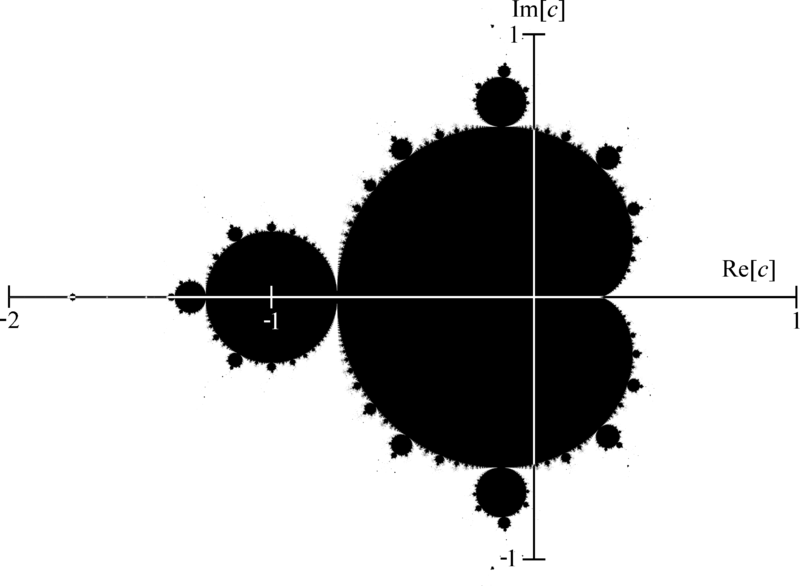
\includegraphics[width=\textwidth]{mandelbrot.png}
	\caption{Die Mandelbrotmenge}
	\label{fig:mandelbrotmenge}
\end{figure}

Weiterhin soll die Hardware durch externe Peripherie konfigurierbar hinsichtlich der angestellten Berechnungen sein. So soll etwa aktuell abgebildete Bereich der Mandelbrotmenge oder auch die Farbgebung der Darstellung im laufenden Betrieb geändert werden können.

Hierfür wurde das FPGA-Trainer Board \textit{Zybo Zynq-7000} zur Verfügung gestellt, welches in %TODO Kapitel linken
genauer vorgestellt wird.

\section{Mitgelieferte Skripte}
%TODO: github repository
Im Git-Repository ... sind sämtliche Python-Skripts, die zur Erstellung von selbsterstellten Bildern verwendet wurden, enthalten. Des weiteren gibt die dort enhaltene Datei \textit{readme.md} Aufschluss über nützliche Skripts, die im Rahmen dieser Arbeit verwendet wurden.

\chapter{Technische Grundlagen}
Zum besseren Verständnis des Gesamtprojektes sollen in diesem Kapitel einige technische Konzepte erläutert werden.

\section{FPGAs}
\label{sec:fpga}
Ein \textit{Field Programmable Gate Array} (kurz FPGA) ist ein Schaltkreis, welcher mit Hilfe von Hardwarebeschreibungssprachen %TODO Kapitel, VHDL erklären
konfiguriert werden kann, um beliebig komplexe logische Schaltungen zu realisieren.\\
Das Grundelement eines solchen Bausteines bilden die sogenannten \textit{Lookup Tables} (kurz LUTs), welche zu einem beliebigen n-bit Input ein 1-bit Output Signal produzieren. Die zugrundeliegende Logiktabelle einer LUT ist hierbei frei programmierbar.

\begin{figure}[H]
	\centering
	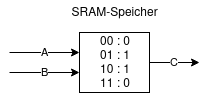
\includegraphics{LUT.png}
	\caption{Beispielhafter Aufbau einer 2-Input LUT}
	\label{fig:LUT}
\end{figure}

Eine LUT, welche die Operation $C = A \oplus B$ implementiert ist in \autoref{fig:LUT} zu sehen. In dieser wird in einem SRAM-Speicher für jede Inputkombination ein Outputwert hinterlegt, wodurch jede 2-Bit Funktion abgebildet werden kann. In Verbindung mit einem Flipflop \footnote{Ein Flipflop ist ein Speicherelement, welches einen einzigen Bit Daten halten kann.} bildet eine LUT dann einen sogenannten Logikblock (s. \autoref{fig:logikblock}).\cite{fpgaDesign}

\begin{figure}[H]
	\centering
	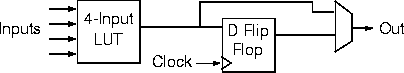
\includegraphics{logic_block.png}
	\caption{Logikblock, aus \cite{fpgaDesign}}
	\label{fig:logikblock}
\end{figure}

Ein FPGA verbindet nun durch ebenfalls konfigurierbare Bussysteme viele solcher Logikblöcke um komplexere Schaltkreise abzubilden.\\
Weiterhin verfügen FPGA-Boards oft noch über ergänzende Hardwarekomponenten, von denen die im Falle dieses Projektes vorhandenen im Folgenden gezeigt werden sollen.

\paragraph{DSP}
Ein \textit{Digitaler Signalprozessor} (DSP) ist ein fest integrierter Baustein, welcher durch Multiplizierer und Akkumulatoren binäre Algorithmen beschleunigt.
So übernimmt dieser etwa grundlegende mathematische Operationen, was dazu führt, dass diese flächen- und energiesparender durchgeführt werden, als bei der Verwendung von LUTs \cite[S. 52]{dsps}.
Typische Anwendungsgebiete dieser Bausteine sind Fließkommamultiplikationen, Schnelle Fourier-Transformationen oder einfache Zähler \cite[S. 14]{dsps}. 
In diesem Projekt wurden die DSPs hauptsächlich aufgrund ihrer 25x18 Bit Multiplizierer verwendet, welche kaskadiert werden können um beliebig Breite Multiplikationen durchzuführen.

\paragraph{Block RAM}
FPGAs verfügen meist über \textit{Block RAM} (BRAM), welcher zur Speicherung binärer Daten dient. Dieser Speicher ist lese-/schreibsynchron, wodurch Inkonsistenzen beim Speicherprozess ausgeschlossen sind \cite[S. 11]{bram}. Um auf diese Speicherblöcke Zugriff zu erlangen muss der von Xilinx mitgelieferte Baustein "Block RAM Generator" verwendet werden.

\paragraph{IO-Komponenten}
Zur Kommunikation mit der Außenwelt verfügen FPGAs über diverse Schnittstellen wie z.B. Knöpfe, Schalter, aber auch komplexere Anbindungen wie etwa VGA (s. hierzu \autoref{sec:vga}) oder PMOD-Anschlüsse.
Diese sind so angebunden, dass ihre Signale direkt in Logikschaltungen von LUTs integriert werden können.
%TODO weitere wichtige komponenten

\section{VGA-Schnittstelle}
\label{sec:vga}
Eine \textit{Video Graphics Array} (VGA) Schnittstelle wird durch einen Videoübertragungsstandard, welcher erstmals von IBM in ihrer \textit{IBM Personal System/2} Modellreihe verbaut wurde, spezifiziert \cite{ibmTimeline}. 
Das Darstellungsverfahren verwendet einen 15-poligen Anschluss, um Videosignale in variabler Auflösung und Bildwiederholungsrate zu übertragen.\\
Hierbei liegen die RGB-Werte eines jeden Pixels als analoge Spannungen an und werden zu bestimmten Zeitpunkten vom Bildschirm ausgelesen. 
Da der VGA-Standard im Jahre 1987 aufkam, war er ursprünglich noch für  Kathodenstrahlröhrenbildschirme (auch Röhrenbildschirme genannt) ausgelegt. 
Die Elektronenstrahlen dieser Bildschirme konnten sich nicht ohne kurze Verzögerungen über die Anzeigefläche bewegen, was bedeutet, dass der VGA-Standard dies berücksichtigt und dem Bildschirm einige $\mu s$ für größere Sprünge des Strahls einräumen muss.
Die größten solchen Sprünge finden statt, wenn eine Pixelreihe übertragen wurde und der Strahl an die erste Pixelposition der nächsten Reihe bewegt werden muss oder wenn das gesamte Bild übertragen wurde und wieder zum oberen linken Pixel gesprungen werden muss.
Während dieser Pausen werden keine RGB-Werte übertragen, man nennt diese zeitlich gedachten Bereiche auch "Porch" (engl. Vorbau).\\

\begin{figure}[H]
	\centering
	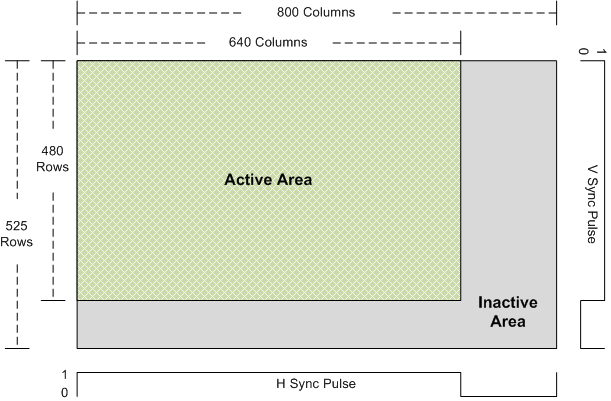
\includegraphics[width=0.8\textwidth]{vga-timing.png}
	\caption{VGA-Timing/Aufbau für eine 640x480 Auflösung, aus \cite{vga-timing}}
	\label{fig:vga}
\end{figure}

Eine 640x480 Pixel Bild baut sich dann wie in \autoref{fig:vga} gezeigt auf:
Zuerst werden 640 Pixel RGB Daten für die erste Reihe empfangen, danach kommen 160 Pixel inaktiver Bereich ($\Rightarrow$ Porch). Das Ende dieses Bereiches wird durch das Ansteigen des low-aktiven Signal HSYNC signalisiert. Dieser Vorgang wird nun 480 mal wiederholt, bis das gesamte Bild übertragen wurde. Draufhin wird analog zur horizonalen Synchronisation das VSYNC Signal für 45 Pixel auf auf 0 gesetzt, um den vertikalen inaktiven zu signalisieren. Die Länge des inaktiven Bereiches setzt sich aus Front-, bzw. Backporch und der Länge des Sync-Pulses zusammen. Die Bedeutungen der einzelnen Signale können fügen jedoch dem nötigen Verständnis nicht mehr hinzu, weswegen die Summe dieser Bereiche als Ganzes angesehen werden kann.
Wie schon erwähnt ist 640x480 jedoch nicht die einzige Auflösung, die mit einem VGA-Anschluss realisierbar ist. Andere Auflösungen (mit anderen Widerholungsraten) müssen vom verwendeten Bildschirm unterstützt sein, und werden durch verschieden schnelle Pixelclocks und Porches realisiert.\\
Die in dieser Arbeit verwendete Auflösung von 800x600 Pixeln bei 60Hz benötigt die in \autoref{tab:vga-timings} dargestellten Werte.

\begin{table}[H]
	\centering
	\begin{tabular}{|l|c|r|}	
		\hline
		aktiver Bereich (horizontal) & Pixel & 800 \\ \hline
		aktiver Bereich (vertikal) & Pixel & 600 \\ \hline
		inaktiver Bereich (horizontal) & Pixel & 256 \\ \hline
		inaktiver Bereich (vertikal) & Pixel & 28 \\ \hline
		Pixelfrequenz & MHz & 40 \\ \hline
	\end{tabular}
	\caption{VGA-Werte für ein 800x600@60Hz Signal}
	\label{tab:vga-timings}
\end{table}

Die in \autoref{tab:vga-timings} gezeigte Pixelfrequenz von 40 MHz bedeutet, dass alle 25 ns ein neuer RGB-Wert anliegen muss. Dies ist ein wichtiger Aspekt für weitere grundliegende Designentscheidungen. %TODO späteres Kapitel hier

\section{Verwendete Hardware}
Zur Umsetzung der Aufgabenstellung wird ein \textit{Zybo Zynq-7000 ARM/FPGA SoC Trainer Board} (fortan kurz Zybo-Board genannt) verwendet (s. \autoref{fig:zybo}).
\begin{figure}[H]
	\centering
	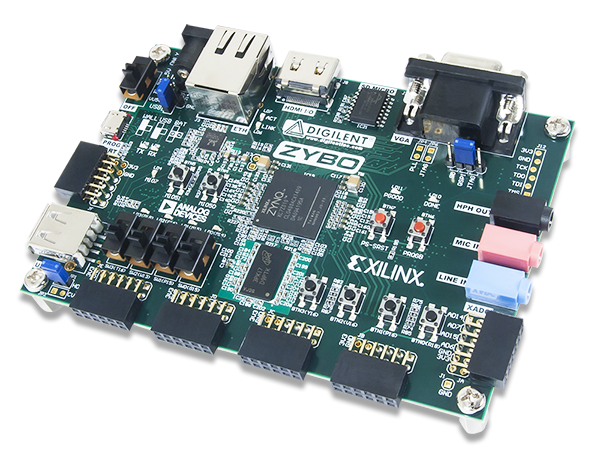
\includegraphics[width=0.8\textwidth]{zybo.png}
	\caption{Zybo Zynq-7000 ARM/FPGA SoC Trainer Board, aus }
	\label{fig:zybo}
\end{figure}
Dieses verfügt unter anderem über folgende technischen Daten:
\begin{itemize}
	\item Xilinx Zynq-7000 FPGA mit 28000 LUTs
	\item 240KB Speicher
	\item 80 DSPs
	\item ARM Cortex-A9 Zweikernprozessor
	\item VGA-Schnittstelle
	\item PMOD-Schnittstellen
\end{itemize}
Der verbaute Zweikernprozessor kommt jedoch im Rahmen dieses Projektes nicht zum Einsatz.

\chapter{Theoretische Grundlagen}
Die dieser Arbeit zugrundelegenden mathematischen Grundlagen und Definitionen sollen in diesem Kapitel näher erläutert werden.

\section{Fraktale}
%todo mandelbrot pole/franz
Der Begriff \textit{Fraktal} wurde vom französischen Mathematiker Benoît Mandelbrot geprägt und leitet sich vom lateinischen Adjektiv \textit{fractus} ab, was \glqq in Stücke gebrochen\grqq{} oder \glqq irregulär\grqq{} bedeutet. Allgmein ist hiermit entweder eine natürlich vorkommende Strukur mit gewissen Eigenschaften oder eine genau definierte mathematische Menge gemeint. \cite[S. 16]{mandelbrot2013fraktale}\\
Für ein intuitives Verständnis des Begriffes sollen im folgenden zuerst einige natürlich vorkommende Fraktale gezeigt werden, woraufhin im nächsten Abschnitt eine formale Definition des Begriffs \textit{Fraktal} folgen soll.

\subsection{Natürlich vorkommende Fraktale}
\label{sec:natfrac}
Fraktale besitzen oft selbstähnliche Strukturen, d.h. dass sich die Gesamtstruktur eines Objektes in kleinerem Maßstab immer wieder findet. Ein Beispiel hierfür ist ein fraktal definierter Baum wie er in \autoref{fig:tree} dargestellt ist. Der Baum wird hierbei über ein einfaches rekursives Verfahren definiert, bei dem immer wieder von jedem Teilbaum aus mit einem festen Winkel in jeweils zwei Äste abgebogen wird.

\begin{figure}[H]
	\centering
	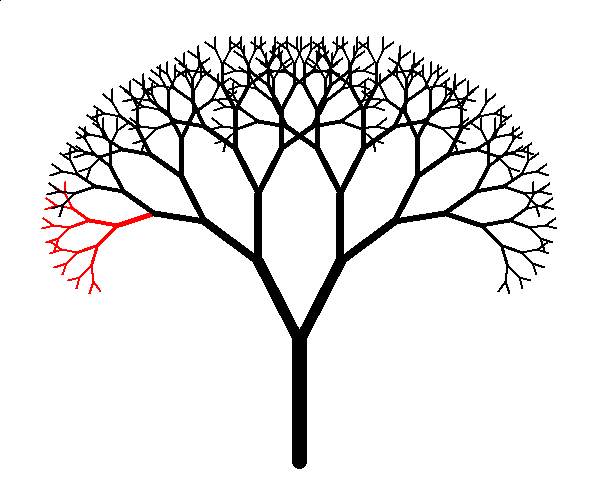
\includegraphics[width=0.6\textwidth]{tree.png}
	\caption{Fraktal definierter Baum, Skript: \textit{baum.py}, abgewandelte Version von \cite{soTree}} %TODO: Skript hinzufügen
	\label{fig:tree}
\end{figure}

Der in \autoref{fig:tree} rot markierte Teilbaum ist in seiner Struktur mit dem Gesamtbaum identisch und besitzt lediglich eine niedrigere rekursive Tiefe.\\
Der Blumenkohl (\autoref{fig:blumenkohl}) ist ein weiteres Beispiel für ein natürlich vorkommendes Fraktal. 
Auch bei diesem wiederholt sich die Gesamtstruktur in kleinerem Maßstab in den Ästen, er besitzt also ein gewisses Maß an Selbstähnlichkeit.

\begin{figure}[H]
	\centering
	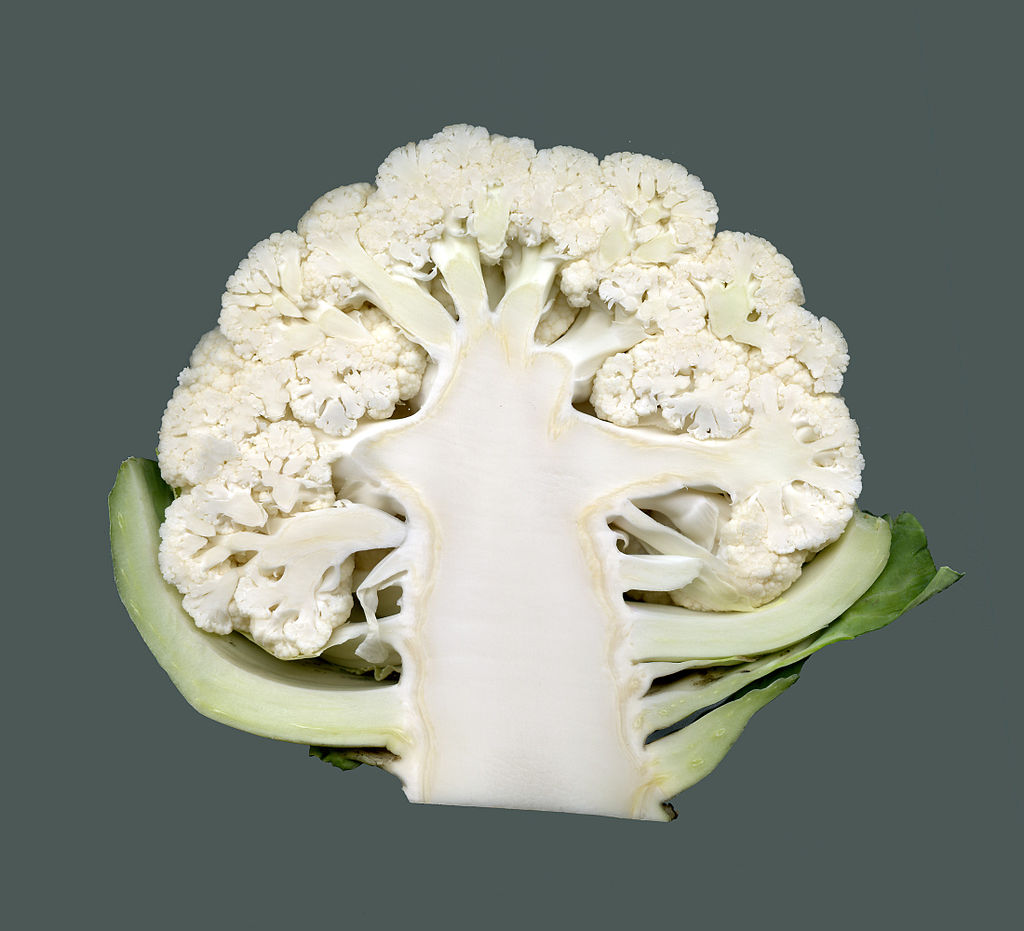
\includegraphics[width=0.4\textwidth]{blumenkohl}
	\caption{Blumenkohl, von Rainer Renz}
	\label{fig:blumenkohl}
\end{figure}

Auch auf höheren Maßstäben, wie etwa bei Bergen oder ganzen Landschaften können Fraktale Strukturen immer wieder beobachtet werden. 
Die relativ einfachen Regeln, die diesen Fraktalen zu Grunde liegen machten sich bereits im Jahre 1980 Computergrafiker wie etwa Loren Carpenter zu Nutzen. Die relativ begrenzten Rechnerleistungen zwangen Animatoren zu diesem Zeitpunkt dazu, komplexe Landschaften Bild für Bild von Hand zu zeichnen. Durch Mandelbrot's Arbeit in fraktaler Geometrie inspiriert animierte Carpenter eine Landschaft für den Film \textit{Star Trek II: The Wrath of Khan}, wobei er hierfür fraktale Verfahren verwendete. \cite{startrekFractals}\\
Die hierfür angestellten Berechnungen waren so simpel, dass pro Bildpunkt nur etwa 20 bis 40 Minuten Rechenaufwand betrieben werden mussten, was einen großen Fortschritt gegenüber der manuellen Animation darstellte. \cite{carpenterVolLibre}\\

\subsection{Fraktale in der Mathematik}
Im Gegensatz zu den in \autoref{sec:natfrac} dargestellten Fraktalen, welche sich auf kleinerer Ebene nur wenige male wiederholen, sind Fraktale in der Mathematik bis zu unendlich hohem Detailgrad definiert.\\
Die formale Definition eines Fraktals lautet hierbei nach Mandelbrot:

\begin{quotation}
	\textit{Ein Fraktal ist nach Definition eine Menge, deren  Hausdorff-Besicovitch Dimension echt die topologische Dimension übersteigt.}
	\\ - Benoît Mandelbrot, aus \cite[S. 27]{mandelbrot2013fraktale}
\end{quotation}
Die hier erwähnte Hausdorff-Besicovitch Dimension ist ein Maß, welches einem beliebigen geometrischen Raum zugeordnet werden kann, wobei die Dimension hier keine natürliche Zahl sein muss. In vereinfachter Form ermittelt sich die Hausdorff-Dimension folgendermaßen:\\
Man betrachte die Anzahl Kugeln (oder Kreisen) $N$ mit Radius $R$, die nötig sind, um eine Punktmenge vollständig abzudecken.
Geht nun $R$ gegen 0 werden immer mehr Kugeln benötigt, um die Punktmenge abzudecken. Beobachtet wird nun in welcher Relation $N$ zu $R$ wächst, mit Hilfe der Formel:
\[D = - \lim_{R \to 0} \frac{\log{N}}{\log{R}}\]
wobei D die Hausdorff-Dimension ist. Betrachtet man etwa eine Linie der Länge 1, kann diese zunächst mit $N = 1$ Kreisen des Radius $R = 1$ abdecken. Halbiert man nun $R$ sind doppelt so viele Kreise nötig um die Linie abzudecken. Allgemein lässt sich sagen, dass in diesem Fall $N$ umgekehrt proportional zu $R$ wächst. Drückt man nun $N$ in Abhängigkeit von R aus erhält man für die Dimension einer Kurve:
\[D = - \lim_{R \to 0} \frac{\log{\frac{1}{R}}}{\log{R}} = 1\]
Analog werden etwa bei einem Rechteck $1/R^2$ Kugeln zur Abdeckung benötigt, wenn $R$ gegen 0 läuft. Die Dimension eines Rechtecks ist daher:
\[D = - \lim_{R \to 0} \frac{\log{\frac{1}{R^2}}}{\log{R}} = 2\]
Bei den hier gezeigten Formen ist die Hausdorff Dimension nicht höher als deren topologische Dimension \footnote{s. hierzu \url{https://www.math.tu-cottbus.de/~froehner/sonstiges/skripte/node9.html}} 
Nimmt man jedoch nun ein Fraktal, wie etwa das Sierpinski-Dreieck %TODO vllt erklären
herbei, hat dieses oft einen gebrochenen Dimensionwert, in diesem Fall:
\[\frac{\log{3}}{\log{2}}\approx 1.585\]
Zusätzlich zu der bereits gezeigten Definition gilt:
Jede Menge, die einen nichtganzzahligen Dimensionwert hat, ist ein Fraktal\cite[S. 27]{mandelbrot2013fraktale}.

\section{Die Mandelbrotmenge}
\label{sec:mandelbrotmath}
Nachdem nun die formale Definition eines Fraktales bekannt ist, soll im folgenden Mandelbrotmenge erläutert werden.\\
Es gilt: Teil der Menge sind alle komplexen Zahlen $c$, für die die Iteration
\[z_0=0\]
\[z_{n+1}=z_n^2 + c\]
nicht divergiert.
Im folgenden sind Iterationen für einige $c$ gezeigt:
\[c_1=1 ; z=2 \rightarrow 5 \rightarrow 26 \rightarrow 677\]
\[c_2=-1 ; z=0 \rightarrow -1 \rightarrow 0 \rightarrow -1\]
\[c_3=1+1i ; z=1+3i \rightarrow -7+7i \rightarrow 1-97i \rightarrow -9407-193i\]

Für $c1$ und $c3$ sieht man schnell, dass der Betrag dieser Zahlen divergiert, während es bei $c2$ klar ist, dass $z$ nur zwischen 0 und -1 wechselt. Also ist $c2$ Teil der Menge, während es $c1$ und $c3$ nicht sind. Jedoch ist die Divergenz nicht für alle Werte so einfach festzustellen. Man betrachte folgendes $c$:
\[c_4=-0.55 + 0.46i ; z=0.45 - 0.04i \rightarrow -0.34 + 0.05i \rightarrow -0.68 + 0.11i \rightarrow -0.09 + 0.29i\]
Hier ist es zunächst unklar ob eine Divergenz stattfinden wird, es müssten erst viele Iterationsschritte angestellt werden, um eine Aussage treffen zu könnnen. Nach 200 Schritten ergibt sich die in \autoref{fig:mandel_c4} gezeigte Struktur, bei der man erkennen kann, dass $z$ gegen einen bestimmten Punkt konvergieren zu scheint.

\begin{figure}[H]
	\centering
	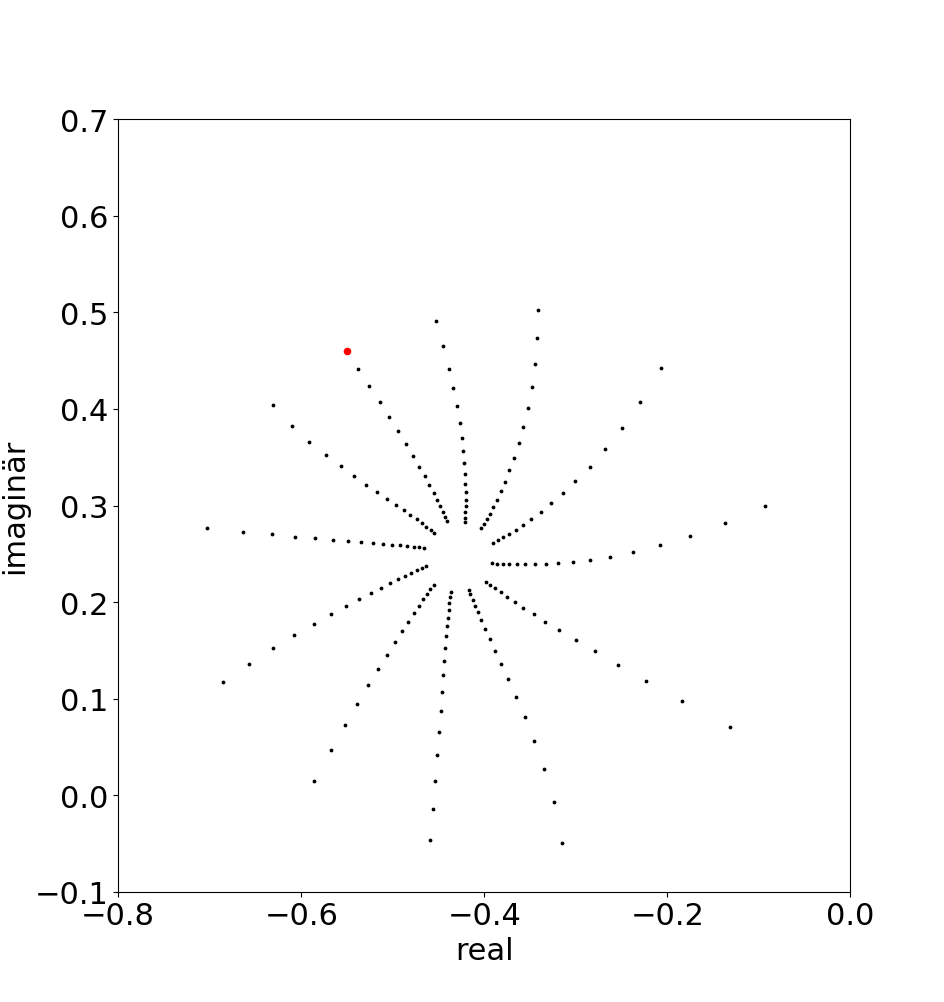
\includegraphics[width=0.44\textwidth]{mandel_c4.png}
	\caption{200 Iterationsschritte für $c = -0.55 + 0.46i$ (rot markierter Punkt)}
	\label{fig:mandel_c4}
\end{figure}

Allgemein gilt, dass ein $c$ nicht zur Mandelbrotmenge gehört, sobald für eine Zahl in einer Iteration gilt \footnote{vgl. hierzu: \cite{mbrotg2}}:
\[|z_n|>2\]
Zählt man nun die Iterationen, die benötigt wurden, um festzustellen, ob eine Zahl divergiert (oder eben konvergiert) und ordnet Bereichen von Iterationszahlen verschiedene Graustufen zu, erhält man ein Bild wie es in \autoref{fig:mandelbrot_1} zu sehen ist.\\
Als Iteration wird fortan der in Zeile 4-7 dargestellte Pseudocode aus \autoref{lst:mandelbrotpseudo} bezeichnet.\\
In der Praxis ist es üblich, sich eine maximale Iterationszahl zu setzen, nach der einfach angenommen wird, dass ein gegebenes $c$ zur Mandelbrotmenge gehört.\\
Eine Funktion zur Berechnung der Iterationszahl eines Punktes $c$ der Mandelbrotmenge wird in \autoref{lst:mandelbrotpseudo} gezeigt.

\begin{lstlisting}[label=lst:mandelbrotpseudo,caption=Algorithmus zur Berechnung der Iterationszahl eines $c$]
funktion mandelbrot(c):
  z = 0
  für iteration in 0 bis maxiter:
 	wenn betrag(z) > 2:
 		return iteration
 	sonst:	
		z = z*z + c
  return iteration //maximale Iteration erreicht
\end{lstlisting}

Diese Funktion würde nun für jeden Pixel (bzw. einem dazugehörigen $c$ Wert) aufgerufen werden, um ein Bild wie in \autoref{fig:mandelbrot_1} darzustellen.

\begin{figure}[H]
	\centering
	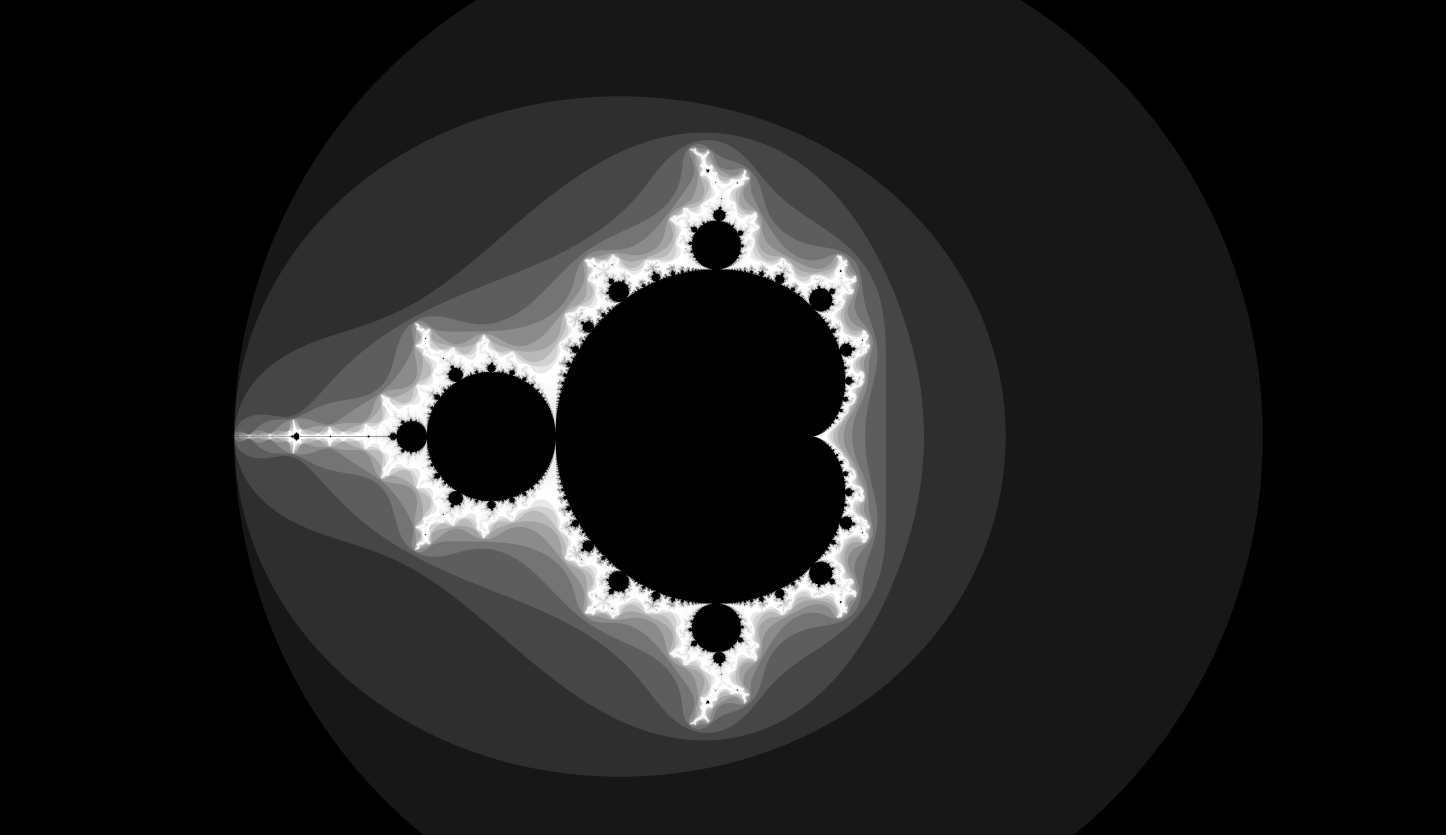
\includegraphics[width=0.65\textwidth]{mandelbrot_4.png}
	\caption{Mandelbrotmenge in Graustufe}
	\label{fig:mandelbrot_1}
\end{figure}

Die eigentliche Faszination der Mandelbrotmenge liegt in ihrem Detailgrad, welcher beim Vergrößern des Randes der Menge (in \autoref{fig:mandelbrot_1} weiß dargestellt), sichtbar wird. Es sind diverse (oft selbstähnliche) Strukturen zu sehen, wobei kein eindeutig visuelles Muster vorhanden zu Sein scheint. Da mit einem Vergrößern des Detailgrades präzisere Berechnungen und höhere maximale Iterationszahlen einhergehen, liegt ein enormer Rechenaufwand vor.\\
Einige besonders sehenswerte Teile der Mandelbrotmenge sind im %ANHANG
dargestellt.

\chapter{Umsetzung} %TODO vllt bessere ÜBerschrift
In diesem Kapitel soll gezeigt werden, wie die in \autoref{sec:aufgabenstellung} formulierte Aufgabenstellung umgesetzt wurde. Hierfür wird zuerst in \autoref{sec:zahlenformat} das für die zugrundeliegenden Berechnungen verwendete Zahlenformat vorgestellt. Danach wird das in \autoref{sec:überblick} gezeigte Gesamtsystem in den folgenden Abschnitten in seinen Einzelteilen erklärt.

\section{Gewähltes Zahlenformat}
\label{sec:zahlenformat}
Die Beobachtung eines komplexzahligen Punktes hinsichtlich seiner Zugehörigkeit zur Mandelbrotmenge setzt ein sehr präzises Datenformat vorraus, damit sich auch bei hohen Vergrößerunsgfaktoren Rechenungenauigkeiten nicht visuell bemerkbar machen.\\
Da die Mandelbrotmenge vollständig in dem in \autoref{tab:minmaxmandel} gezeigten Bereich liegt, muss das verwendete Datenformat nur einen kleinen Teil seiner Bits für den ganzzahligen Teil der verschiedenen Berechnungen verwenden. \\

\begin{table}[H]
	\centering
	\begin{tabular}{|l|r|}	
		\hline
		Minimum Realteil & -2 \\ \hline
		Maximum Realteil & 0.5 \\ \hline
		Minimum Imaginärteil & -1.25i \\ \hline
		Maximum Imaginärteil & 1.25i \\ \hline
	\end{tabular}
	\caption{Bereich der Mandelbrotmenge}
	\label{tab:minmaxmandel}
\end{table}

Der große Teil des Bitvektors sollte also für die Darstellung der Nachkommastellen verwendet werden.
Die Sprache VHDL liefert im Packet \textit{IEEE\_numeric\_std} den Typ \textit{signed}, welcher dazu dient vorzeichenbehaftete Ganzzahlen in einem beliebig breiten Bitvektor darzustellen. \footnote{s. hierzu die Definition in: \cite{ieeeNumeric}}.\\
Da die Rechenoperationen auf binärer Ebene für eben solche Festkommazahlen und Ganzzahlen (jeweils mit Vorzeichen) identisch sind, ist der signed-Typ gut zur Verwendung geeignet.
Intern rechnet das FPGA also mit großen Ganzzahlen, welche jedoch eigentlich Festkommazahlen repräsentieren.\\
Hierbei gilt es, die Breite der signed Zahlen so festzulegen, dass zum einen eine maximale Präzision erreicht wird und zum Anderen die mit ihnen durchgeführten Multiplikationen von den eingebauten DSPs durchgeführt werden können (s. \autoref{sec:fpga}).\\
Durch Testen ergab sich, dass Multiplikationen mit mehr als 40 Bit durch LUTs umgesetzt werden (statt durch DSPs), weswegen eben diese 40 Bit sich als ideale Breite herausstellten.\\
Da der Betrag einer Komplexen Zahl am Anfang einer Iteration nicht größer als 2 sein kann (dies wird stets geprüft), ist das größte Multiplikationsergebnis $2*2=4$, weswegen $\log_24+1=3$ Bits für den Vorkommateil der Zahl benötigt werden.\\
Das höchstwertige Bit ist für das Vorzeichen reserviert, weswegen 36 Bits für den Nachommateil bleiben. Hiermit ist die Genauigkeit im Dezimalsystem ungefährt 11 Stellen:
\[36 * log_{10}2 \approx 10.84\]
Die betragsmäßig kleinste darstellbare Zahl ist damit:
\[0000,0000...001_2 = 2^{-36} \approx 1.455_{10}*10^{-11} \]
Die betragsmäßig größte darstellbare Zahl ist also:
\[0111,1111...111_2 = 8 - 2^{-36} \approx 7.99999999998 \]
Die Zahl wird im Einerkomplement dargestellt, was bedeutet, dass bei negativen Zahlen alle Bits invertiert werden. So ist die kleinste darstellbare Zahl:
\[1000,0000...000_2 = -8 + 2^{-36} \approx -7.99999999998 \]
%TODO: skript hinzufügen
Selbst bei einer 134217728-fachen Vergrößerung (27 Zooms um Faktor 2) ergeben sich mit dieser Präzision noch keine visuell wahrnehmbaren Rechenfehler.\\
Um noch tiefere Zooms zu realisieren müsste entweder eine variable Breite der einzelnen Datenworte realisiert werden, oder der grundlegende Algorithmus zur Berechnung der Mandelbrotmenge geändert werden.
Hierfür würde sich der relativ neue Algorithmus von K.I. Martin (s. \cite{SUPERFRACTALTHINGMATHS}) eignen, welcher größtenteils unabhängig von aktueller Zoomtiefe und ohne die Verwendung von beliebig präzisen Datentypen auskommt \cite{SUPERFRACTALTHINGMATHS}.\\
Da die Umsetzung dieses Algorithmus jedoch um einiges komplexer als die in dieser Arbeit verwendete Methode ist und die aktuelle Präzision zufriedenstellend ist, wird von dessen Imlmentierung abgesehen, jedoch ist die Bitbreite der einzelnen Datenworte in der Datei \textit{constants.vhd} konfigurierbar.
\paragraph{Bitbreite bei Multiplikationen}
Da bei der Multiplikation zweier 40-Bit-Zahlen das Ergebnis 80 Bit lang ist, muss dieses wieder in ein 40-Bit Format zurückgeführt werden.
Dies geschieht mittels einer dafür entwickelten VHDL-Prozedur \textit{fixlen}, welche in der Datei %TODO Datei hier
zu finden ist.

\begin{figure}[H]
	\centering
	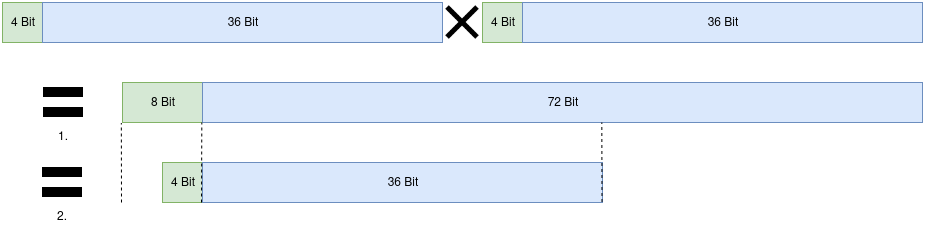
\includegraphics[width=\textwidth]{mulfixlen.png}
	\caption{Funktionsweise der Funktion \textit{fixlen}}
	\label{fig:fixlen}
\end{figure}

Die Funktionsweise dieser Prozesdur ist in \autoref{fig:fixlen} dargestellt.
Die aus der Multiplikation in Schritt 1. entstehende 80 Bit zahl besteht aus 8 Bits Vorkommateil und 72 Bit Nachkommateil.
Um diese Zahl nun wieder in das normale Format zurückzuführen werden die ersten 4 Bit des Vorkommateils und die letzten 36 Bits des Nachkommateils abgeschnitten (Schritt 2.).\\
Hierbei verliert das Ergebnis der Multiplikation an Präzision, was jedoch unvermeidbar ist, da sich die Länge der Datenworte sonst bei jeder Multiplikation verdoppeln würde.\\
Umgesetzt wird dieses Verfahren in einer VHDL-Funktion \textit{fixlen} (\autoref{lst:fixlen}), welche durch die Konstante \textit{N\_BITS} parametrisierbar ist.
%TODO: Dateireferenz
\begin{lstlisting}[label=lst:fixlen,caption=VHDL-Funktion \textit{fixlen}]
--N_BITS sei hier 16
function fixlen (input : signed(N_BITS*2-1 downto 0)) return signed is
	variable ret : signed(N_BITS-1 downto 0);
begin
	ret := input(N_BITS*2-1-4 downto N_BITS*2-4-N_BITS);
	return ret;
end fixlen;

a <= "1111000011110000";
b <= "0000111100001111";

a <= a*b; --Fehler!
a <= fixlen(a*b);
\end{lstlisting}
Da das Ergebnis der 16-Bit Multiplikation in Zeile 10 32 Bit breit ist, kann dieses nicht dem 16-Bit Wert \textit{a} zugewiesen werden.
Stattdessen muss dieses Ergebnis wie in Zeile 11 gezeigt wieder auf eine Breite von 16 Bit gekürzt werden.

\paragraph{Umwandlung zwischen Zahlensystemen}
Die Verfahren zur Umwandlung zwischen dem im Rahmen dieser Arbeit vorgestellten Zahlensystem und dem Dezimalsystem soll im folgenden aufgezeigt werden.
%TODO schreiben 

\section{Systemüberblick}
\label{sec:überblick}
In diesem Abschnitt soll ein Überblick über das entwickelte Gesamtsystem gegeben werden, während in den folgenden Abschnitten die einzelnen Komponenten erläutert werden.

\begin{figure}[H]
	\centering
	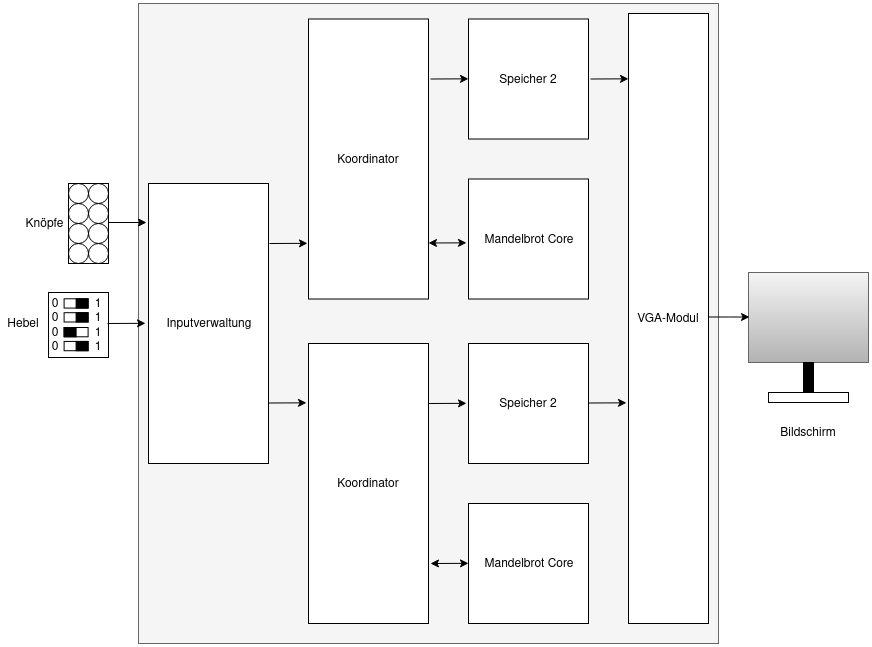
\includegraphics[width=.8\textwidth]{top.png}
	\caption{Gesamtsystem mit 2 Kernen}
	\label{fig:top}
\end{figure}

%TODO in bildern mandelbrot-core (bindestrich)
In \autoref{fig:top} ist der konzeptuelle 2-kernige Aufbau des Gesamtsystems dargestellt.\\
Die Darstellung erfolgt über eine VGA-Schnittstelle, welche durch das VGA-Modul bedient wird.
Dieses liest stetig Pixelwerte aus den vorhandenen Speicherblöcken aus und generiert aus diesen ein gültiges VGA-Signal.\\
Der Speicher wird wiederum von den sogenannten \textit{Koordinatoren} gefüllt.
Jeder Koordinator verwaltet die Berechnungen eines \textit{Mandelbrot-Cores} und schreibt dessen Rechenergebnisse in seinen eigenen Speicher.\\
Die Koordinatoren erhalten Informationen wie z.B. den aktuell darzustellenden Bereich von der Inputverwaltung, welche die externen Peripheriegeräte wie Hebel und Knöpfe verwaltet.\\

\section{Komponentenbeschreibung}
Die genaue Funktion und Umsetzung aller genannten Module wird in den folgenden Abschnitten gezeigt.
Alle Signale der vorgestellten Bauteile sind high-aktiv,
%todo: erklären?
wenn dies nicht der Fall ist, wird es explizit deklariert.
Zudem sind alle Inputs/Outpus \textbf{fettgedruckt}, um sie von Variablen in Gleichungen unterscheiden zu können.

\subsection{Mandelbrot-Core}
\label{subsec:mandelcore}
Der zentralste Baustein des Chips ist der Mandelbrot-Core (s. \autoref{fig:schem_mandelbrotcore}), welcher für ein gegebenes $c$ einen Iterationswert errechnet.
\begin{figure}[H]
	\centering
	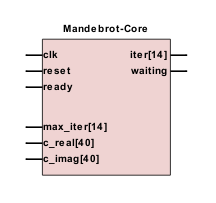
\includegraphics[width=0.35\textwidth]{schem_mandelbrotcore.png}
	\caption{Mandelbrot-Core, schematische Darstellung}
	\label{fig:schem_mandelbrotcore}
\end{figure}
Als Input erhält ein Mandelbrot-Core zunächst die üblichen Clock- und Resetsignale (\textbf{clk},\textbf{reset}).
Des weiteren liegt der zu untersuchende Punkt $c$ an den Eingängen \textbf{c\_real} (Realteil) und \textbf{c\_imag} (Imaginärteil) an.
Die maximale Zahl von Iterationen, nach der angenommen wird, dass ein Punkt nicht zur Mandelbrotmenge gehört wird über das Eingangssignal \textbf{max\_iter} übermittelt.\\
Sobald über das Signal \textbf{ready} angezeigt wird, dass \textbf{c\_real}, \textbf{c\_imag} und \textbf{max\_iter} stabil anliegen beginnt der Kern den Iterationsvorgang.\\
Hierbei wird jeden Zyklus von \textbf{clk} eine Iteration abgeschlossen.\\
Über den Ausgang \textbf{waiting} wird angezeigt, dass ein endgültiges Ergebnis am Ausgang \textbf{iter} anliegt und der Kern bereit für neue Inputs ist.
Das Ergebnis kann Werte zwischen (jeweils inklusive) 0 (falls $|c|>2$) und \textbf{maxiter} annehmen.\\
\autoref{fig:wave_mandelbrotcore} zeigt ein Impulsdiagramm der In- und Outputs eines Mandelbrot-Cores.
Zu bestimmten ist in diesem Fall die Iterationszahl für den Punkt $-0,7487-0,7487i$, wobei die maximale Iterationszahl 100 sein soll.
Diese Werte werden an die Inputs \textbf{c\_real},\textbf{c\_imag} und \textbf{max\_iter} angeleg.
Sobald diese stabil vorliegen, wird dies durch einen Puls des Signales \textbf{ready} signalisiert, wodurch der Core seine Berechnungen startet.
Nach einigen Zyklen des Clocksignals liegt dann die Iterationszahl (in diesem Fall 3) am Ausgang \textbf{iter} an.
\begin{figure}[H]
	\centering
	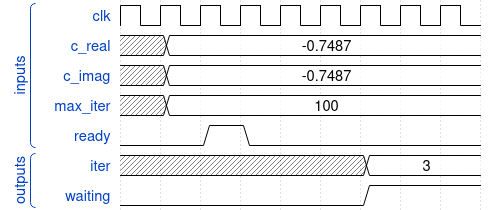
\includegraphics[width=.8\textwidth]{wave_mandelcore.png}
	\caption{Funktionsweise Mandelbrot-Core, Impulsdiagramm}
	\label{fig:wave_mandelbrotcore}
\end{figure}
Vor diesem Zeitpunkt ist der Zustand von \textbf{iter} undefiniert, erst nach der steigenden Taktflanke von \textbf{waiting} liegt das richtige Ergebnis an.
Ab diesem Zeitpunkt ist der Core auch wieder bereit, neue Werte von $c$ zu verarbeiten.\\
Da der Mandelbrot-Core über einen den Eingang \textbf{max\_iter} verfügt und diesen auch bei jeder Berechnung neu ausliest, kann die maximale Iterationszahl im laufenden Betrieb jederzeit geändert werden,
\footnote{Neue Werte für die Signale \textbf{c\_real}, \textbf{c\_imag} und \textbf{max\_iter} werden erst beim nächsten \textbf{ready} Puls übernommen}
was nützlich ist um bei steigender Vergrößerungsstufe den Detailgrad der Berechnung erhöhen zu können.\\
Die Mandelbrot-Cores werden mit einer eigenen Clock, die unabhängig von z.B. der VGA-Clock läuft, getaktet.
Die maximal mögliche Taktrate ist hierbei abhängig von der Anzahl der Rechenschritte, die in jedem Iterationsschritt durchgeführt werden müssen.
Eine Iteration besteht aus folgenen Bestandteilen:
\begin{enumerate}[label=(\Alph*)]
	\item Überprüfen, ob maximale Iterationszahl bereits erreicht ist, wenn dem so ist,ist die Berechnung abgeschlossen
	\item Wenn nicht, berechne neuen Wert für $z$, falls dieser größer als 2 ist, ist die Berechnung abgeschlossen
	\item Zeige den aktuellen Zustand der Berechnung über die Signale \textbf{waiting} und \textbf{iter} an
\end{enumerate}
Die Abfrage (A) der aktuellen Iterationszahl und der Vergleich mit der maximal zulässigen ist hierbei sehr trivial und nimmt deshalb auch keine nennenswerte Zeit in Anspruch, muss also auch nicht weiter optimiert werden.\\
Der komplexzahlige Iterationsteil (B) besteht jedoch aus mehreren Multiplikationen, Additionen und Vergleichen, weswegen hier ein großer Teil der pro Iteration entstehenden Verzögerung entsteht.
Es gilt, diesen Bestandteil (B) weitesgehend zu optimieren, was durch einfache algebraische Umformungen geschehen kann.\\
In jedem Schritt muss überprüft werden, ob $z$ kleiner 2 ist:
\[abs(z) <= 2\]
Der Betrag (abs) einer komplexen Zahl mit Realteil $z_r$ und Imaginärteil $z_i$ ist als ihr Abstand vom Ursprung definiert:
\[abs(z) = \sqrt{z_r^2 + z_i^2}\]
Also muss geprüft werden, ob gilt:
\[\sqrt{z_r^2 + z_i^2} <= 2\]
Das Ziehen der Wurzel kann in diesem Fall durch das Quadrieren beider Seiten umgangen werden:
\begin{equation}
	\label{eq:bedingung}
	z_r^2 + z_i^2 <= 4
\end{equation}
Falls dies wahr ist, muss der Wert von $z$ aktualisiert werden und die Iterationszahl kann um eins erhöht werden:
\[z_{n+1} = z_n^2 + c\]
\[iter = iter + 1\]
Das Quadrat einer komplexen Zahl mit Realteil $a$ und Imaginärteil $b$ wird folgendermaßen berechnet:
\[(a + bi)^2 = a^2 + 2abi + b^2*i^2 = a^2 + 2abi - b^2\]
Im Fall von $z$ gilt also:
\[z^2+c=(z_r + z_ii)^2 = z_r^2 - z_i^2 + 2z_rz_ii + c\]
Da die Bestandteile der komplexen Zahlen getrennt gespeichert sind, müssen diese isoliert betrachtet werden (das = Zeichen ist in diesem Kontext als Zuweisungsoperator zu verstehen):
\begin{equation}
	\label{eq:zr}
	z_r = z_r^2 - z_i^2 + c_r
\end{equation}
\begin{equation}
	\label{eq:zi}
	z_i = 2z_rz_ii + c_i = z_rz_ii + z_rz_ii + c_i
\end{equation}
Die Quadrate von $z_r$ und $z_i$ kommen sowohl in \autoref{eq:bedingung} als auch in \autoref{eq:zr} vor, müssen aber nur ein mal berechnet werden, was zwei Multiplikationen spart.\\
Auch das Ersetzen der Multiplikation mit zwei in \autoref{eq:zi} durch eine Addition erspart eine Multiplikation.
Der nicht optimierte Iterationsschritt (B) enthält eine Wurzel, sechs Multiplikationen und vier Additionen.
Durch Wiederverwenden bereits berechneter Werte und algebraische Optimierung sind nun lediglich 3 Multiplikationen und fünf Additionen nötig.\\
Das optimierte Iterationsverfahren läuft bei einer maximalen Clockfrequenz von 40MHz stabil, was bedeutet dass eine einzelne Iteration maximal 25ns in Anspruch nimmt.

\subsection{Mandelbrot-Koordinator}
Der in \autoref{fig:schem_mandelbrotkoord} gezeigte Mandelbrot-Koordinator verwaltet einen Mandelbrot-Core und schreibt dessen Ergebnisse in den in \autoref{subsec:ram} beschriebenen RAM.

\begin{figure}[H]
	\centering
	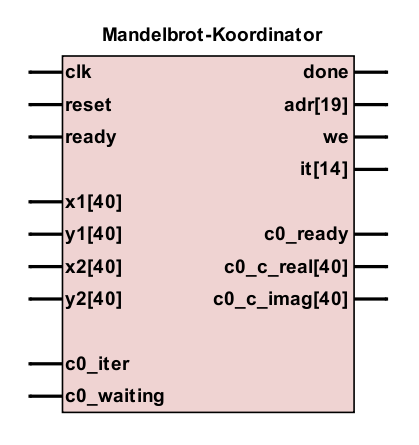
\includegraphics[width=0.35\textwidth]{schem_mandelkoord.png}
	\caption{Mandelbrot-Koordinator, schematische Darstellung}
	\label{fig:schem_mandelbrotkoord}
\end{figure}
Berechnet wird die Mandelbrotmenge in dem durch die Punkte (\textbf{x1}/\textbf{y1}) und (\textbf{x2}/\textbf{y2}) aufgespannten Rechteck (s. \autoref{fig:mandelcoordpixels}).
Liegen diese Eingangssignale stabil an, kann durch das Aktivieren des Eingangs \textbf{ready} der Rechenvorgang gestartet werden.

\begin{figure}[H]
	\centering
	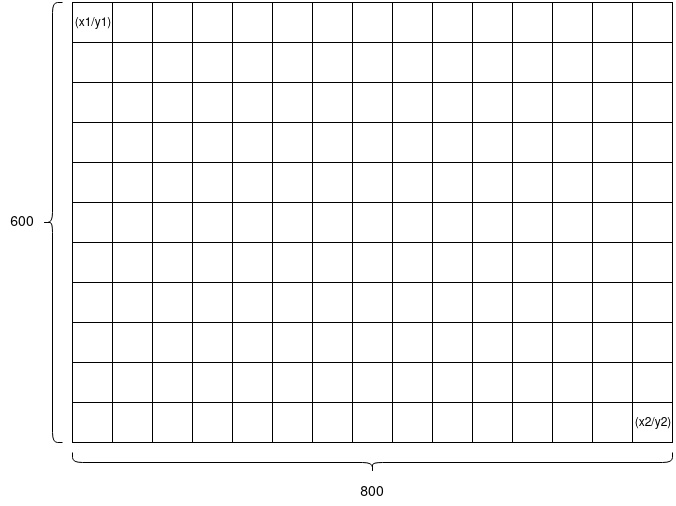
\includegraphics[width=.8\textwidth]{mandelcoord.png}
	\caption{Mandelbrot-Koordinator, schematische Darstellung}
	\label{fig:mandelcoordpixels}
\end{figure}
Der obere linke Pixel repräsentiert den Punkt (\textbf{x1}/\textbf{y1}).
Um zu einer gegebenen Pixelkoordinate ($p_x/p_y$) den zugehörigen komplexzahligen Punkt ($c_r/c_i$) zu finden wird folgende Formel verwendet:
\[c_r = \mathbf{x1} + step_x * p_x\] 
\[c_i = \mathbf{y1} + step_y * p_y\]
mit:
\[step_x = \frac{x2-x1}{800}\]
\[step_y = \frac{y2-y1}{600}\]
Damit das dargestellte Bild nicht gestaucht ist, sollte das Seitenverhältnis von 800x600 Pixeln eingehalten werden:
\[\frac{x2-x1}{y2-y1}=\frac{4}{3}\]
Wenn die Mandelbrotmenge beispielsweise für das Rechteck mit den Eckpunkten (-2/-2) und (2/1) dargestellt werden soll gilt:
\[step_x = \frac{2-(-2)}{800} = 0,005\]
\[step_y = \frac{1-(-2)}{600} = 0,005\]
Dem Pixel (250/100) würde folgender Punkt $c: -0,75 -1,5i$ zugeordnet werden:
\[c_r = -2 + 0,005 * 250 = -0,75\] 
\[c_i = -2 + 0,005 * 100 = -1,5\]
Diese Werte werden an die zugehörigen Outputsignale \textbf{c0\_c\_real} und \textbf{c0\_c\_imag} angelegt und anschließen durch Aktivieren des Ausgangs \textbf{c0\_ready} bestätigt.\\
Im Anschluss wartet der Mandelbrot-Koordinator bis das Eingangssignal \textbf{c0\_waiting} aktiv wird und schreibt den an \textbf{c0\_iter} anliegenden Wert in den RAM.\\
Hierfür werden die Signale \textbf{adr},\textbf{we} und \textbf{it} verwendet,wobei deren genaue Funktionsweise im Kapitel
%TODO: linken
näher erläutert wird.
Wenn jeder Pixel abgearbeitet wurde, wird dies durch das Signal \textbf{done} signalisiert und der Koordinator ist bereit, neue Eingangssignale aufzunehmen.\\
%TODO: State-Machine

\subsection{Speicher}
\label{subsec:ram}
\begin{figure}[H]
	\centering
	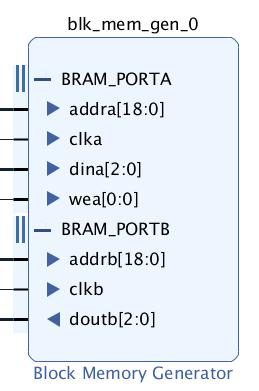
\includegraphics[width=0.25\textwidth]{blockram.jpg}
	\caption{Block Memory Generator, IP-Bauteil}
	\label{fig:schem_bram}
\end{figure}
Der Block Memory Generator ist ein mit Vivado %TODO erklären
mitgeliefertes IP-Bauteil, welches ermöglicht den auf FPGA-Boards verfügbaren Block-RAM zu verwenden.\\
Verwendet wird der Block-RAM im Rahmen dieses Projekts, um die Iterationswerte, die jedem Pixel zugeordnet werden (s. \autoref{subsec:mandelcore}) zu speichern.\\
Der Block-RAM des Zybo-Board setzt sich aus 60 32768-Bit RAMB18E1-Blöcken zusammen, verfügt also über 1966080 Bit (240 KB) Speicher \cite[S. 14]{bram} \cite{zyboref}.
Da in diesem Speicher ein 800x600 Pixel Bild gespeichert (und ausgelesen) werden soll, ergeben sich 4 Bit Speicher pro Pixel:
\[\floor{\frac{1966080 Bit}{800*600 Pixel}}=4 \frac{Bit}{Pixel} \]
Ein Datenwort in diesem Speicher kann also 16 ($2^4$) Zustände annehmen, wodurch 16 verschiedene Farbwerte gespeichert werden können.\\
Um alle Datenworte adressieren zu können wird ein 19-Bit Adresswort benötigt:
\[\ceil{log_2{(800*600)}}=19\]
Da die Mandelbrot-Koordinatoren einen 14-Bit Iterationswert liefern, muss dieser zur Einspeicherung auf eine Breite von 4 Bit gemappt werden. Diese Problemstellung wird in \autoref{subsec:luts} behandelt.\\
Im Betrieb wird der Speicher permanent vom VGA-Modul ausgelesen, während die Mandelbrot-Koordinatoren neue Werte im Speicher ablegen. Da die Synchronisation dieser beiden Vorgänge enorm aufwändig wäre und die Anzahl der Lese-/Schreibzugriffe pro Sekunde eingeschränken würde, muss der Speicher im sog. \textit{Dual-Port}-Modus betrieben werden.\\
Ein Speicher im Dual-Port-Modus verfügt über zwei Ports, welche völlig unabhängig voneinander agieren (\textbf{BRAM\_PORTA}, \textbf{BRAM\_PORTB}; fortan \textbf{Port A} bzw. \textbf{Port B} genannt). 
Jeder dieser Ports verfügt über einen eigenen Takt (\textbf{clka},\textbf{clkb}) und einen eigenen Adressbus.
\textbf{Port A} wird rein zum Schreibzugriff verwendet, während \textbf{Port B} rein zum Lesezugriff konfiguriert ist. Dies äußert sich darin, dass \textbf{Port A} einen \textit{Write Enable}-Eingang (Schreibzugriffsaktivierung) \textbf{wea} hat, jedoch keinen Datenausgang. 
\textbf{Port B} verfügt wiederum über einen Datenausgang \textbf{doutb}, jedoch über %TODO: hier weiter
\subsection{Lookup Tables}
\label{subsec:luts}
Lookup Tables (kurz LUTs) sind Bausteine, welche für einen Index $i$ einen bestimmten Tabelleneintrag als Output liefern können.
Die Tabelleneinträge sind hierbei vordefiniert, was einige Berechnungen, die sonst in Hardware durchgeführt werden müssten, erspart.\\
Im folgenden werden die im Rahmen dieses Projekts %$TODO: projekts/Projektes nachschauen
verwendeten LUTs vorgestellt.\\
Da in dem in \autoref{subsec:ram} beschrieben Speicher nur 4-Bit Datenworte gespeichert werden können, ist es nicht möglich, für jeden einzelnen Pixel RGB-Werte zu hinterlegen, da diese auf dem Zybo-Board 16 Bit breit sind \cite{zyboref}. Es muss also eine Farbtabelle existieren, welche von 4-Bit Iterations-Werten auf 16-Bit RGB-Werte übersetzt (\textbf{LUT1}).\\
Da der Mandelbrot-Koordinator 14-Bit Iterationswerte liefert, der Speicher jedoch nur 4-Bit %TODO: bitschreibweise konsistent
Datenworte speichern kann, muss auch hier eine Übersetzung stattfinden (\textbf{LUT2}).\\
Für die Umsetzung von \textbf{LUT2} wird folgende Formel verwendet:
\[I_F = \ceil{\frac{i}{i_{max}}*15}\]
Hierbei sind $i$ und $i_{max}$ 14-Bit Zahlen, wobei $I_F$ eine 4 Bit Zahl ist, wodurch $I_F$ in den Speicher geschrieben werden kann.\\
Beim Auslesen wird wiederum \textbf{LUT1} verwendet, um die per VGA dargestellten RGB-Werte zu erhalten.
Die verwendeten RGB-Werte sind in einer frei konfigurierbaren %datei linken
Farbtabelle hinterlegt.
Sei die maximale Iterationszahl $i_{max} = 100$.
Zur Ermittlung der Farbe eines Pixels muss zunächst der Farbindex $I_F$ errechnet werden. Wenn etwa 33 Iterationen genötigt wurden sieht ergibt sich:
\[I_F = \ceil{\frac{33}{100}*15} = \ceil{4,95} = 5\]
Nun kann der zugehörige RGB-Wert aus einer Farbtabelle (z.B. \autoref{tab:farben}) entnommen und an das VGA-Modul weitergeleitet werden\footnote{Die hier dargestellten RGB-Werte sind 24 Bit breit, da dies die übliche RGB-Notation ist. Die RGB-Werte auf dem Zybo-Board sind nur 16 Bit breit.}:

\begin{table}[H]
	\centering
	\begin{tabular}{ll}
		\begin{tabular}{|c|c|}
			\hline
			Index $I_F$ & Farbe(RGB)	\\ \hline
			0	& \colorbox[RGB]{255,0,0}		{\#FF0000}\\ \hline
			1	& \colorbox[RGB]{238,17,0}		{\#EE1100}\\ \hline
			2	& \colorbox[RGB]{221,34,0}		{\#DD2200}\\ \hline
			3	& \colorbox[RGB]{204,51,0}		{\#CC3300}\\ \hline
			4	& \colorbox[RGB]{187,68,0}		{\#BB4400}\\ \hline
			5	& \colorbox[RGB]{170,85,0}		{\#AA5500}\\ \hline
			6	& \colorbox[RGB]{153,102,0}		{\#996600}\\ \hline
			7	& \colorbox[RGB]{136,119,0}		{\#887700}\\ \hline
		\end{tabular}

		\begin{tabular}{|c|c|}
			\hline
			Index $I_F$ & Farbe(RGB)	\\ \hline
			8	& \colorbox[RGB]{119,136,0}		{\#778800}\\ \hline
			9	& \colorbox[RGB]{102,153,0}		{\#669900}\\ \hline
			10	& \colorbox[RGB]{85,170,0}		{\#55AA00}\\ \hline
			11	& \colorbox[RGB]{68,187,0}		{\#44BB00}\\ \hline
			12	& \colorbox[RGB]{51,204,0}		{\#33CC00}\\ \hline
			13	& \colorbox[RGB]{34,221,0}		{\#22DD00}\\ \hline
			14	& \colorbox[RGB]{17,238,0}		{\#11EE00}\\ \hline
			15	& \colorbox[RGB]{0,255,0}		{\#00FF00}\\ \hline
		\end{tabular}
	\end{tabular}
	\caption{Farbtabelle, Übergang von Rot nach Grün }
	\label{tab:farben}
\end{table}
%TODO: implmentierte Farbtabellen, auch in den Anhang

\subsection{VGA-Modul}
\label{subsec:vga-modul}
\begin{figure}[H]
	\centering
	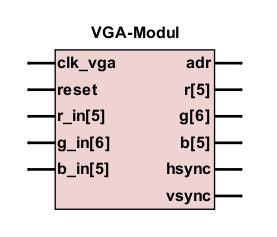
\includegraphics[width=0.4\textwidth]{schem_vga.png}
	\caption{Aufbau des VGA-Moduls}
	\label{fig:schem_vga}
\end{figure}
Das VGA-Modul (s. \autoref{fig:schem_vga}) setzt das in \autoref{sec:vga} beschriebene Videosignal (800x600 Pixel bei 60 Bildern pro Sekunde) um.\\
Hierfür wurde das VGA-Modul aus \cite{vgagit} an das Zybo-Board angepasst.
Intern führt das VGA-Modul stets zwei Zähler $x$ und $y$, welche die Position des gerade zu beschreibenden Pixels halten.
Mit Hilfe der auf diesen Positionsdaten beruhenden Formel wird die aktuell auszulesende Adresse im Speicher berechnet:
\[\mathbf{adr}= y*800+ x\]
Sobald diese Adresse an den Output \textbf{adr} angelegt wird, liegen die korrekten RGB aus dem Speicher\footnote{Der Speicher hält 4-Bit Iterationswerte, welche von den in \autoref{subsec:luts} vorgestellten LUTs in RGB-Werte übersetzt werden.} an den Inputs \textbf{r\_in},\textbf{g\_in} und \textbf{b\_in} an.
Diese Signale werden dann direkt an die Ausgänge \textbf{r},\textbf{g} und \textbf{b} weitergeleitet.\\
Um mit dem Bildschirmtakt synchron zu arbeiten werden die Signale \textbf{hsync} bzw. \textbf{vsync} wie in \autoref{sec:vga} beschrieben betrieben.\\
Da die in \autoref{sec:peripheriesteuerung} vorgestellte Steuerung stets den Mittelpunkt des Bildschirms als Referenzpunkt verwendet, ist es nützlich diesen zu kennzeichnen.
Dies geschieht durch ein Farbenkreuz, welches aus zwei roten Linien besteht (s. \autoref{fig:fadenkreuz}).
\begin{figure}[H]
	\centering
	\includegraphics[width=0.8\textwidth]{fadenkreuz.jpg}
	\caption{Ausschnitt der Mandelbrotmenge mit Fadenkreuz}
	\label{fig:fadenkreuz}
\end{figure}
Dieses Fadenkreuz wird vom VGA-Modul erzeugt, indem immer, wenn eine der folgenden Bedingungen erfüllt ist, ein rein roter RGB-Wert an den Bildschirm gesendet wird:
\begin{itemize}
	\item Horizontale Position gleich 309 UND vertikale Position zwischen 289 und 309
	\item Vertikale Position gleich 409 UND horizonale Position zwischen 389 und 409
\end{itemize}

\section{Peripherie und Steuerung}
\label{sec:peripheriesteuerung}
Die Darstellung lässt sich über die an einer PMOD-Schnittstelle angeschlossenen Knöpfe manipulieren.
Alle Inputs werden vom Input-Modul (\autoref{fig:schem_input}) verwaltet:
\begin{figure}[H]
	\centering
	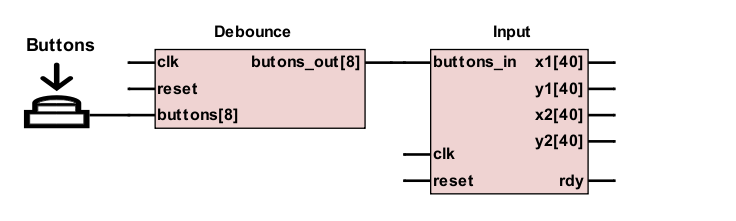
\includegraphics[width=0.8\textwidth]{input.png}
	\caption{Debouncer und Input-Modul, schematische Darstellung}
	\label{fig:schem_input}
\end{figure}
%TODO: vllt alle darstellungen deutsch("Buttons")
Das Input-Modul fragt zu jedem Takt von \textbf{clk} den Zustand der Knöpfe vom Debouncer ab.
Wenn einer (oder mehrere) Knöpfe gedrückt sind wird eine der folgenden Aktionen ausgeführt:
\begin{itemize}
	\item Bewegen des Bildbereichs
	\item Vergrößern/Verkleinern des aktuellen Ausschnitts
	\item Ein-/Ausschalten Hochauflösungsmodus
\end{itemize}
Für das Bewegen des Bildbereichs werden vier Knöpfe verwendet.
Ein Drücken dieser Knöpfe bewirkt, dass der gesammte dargestellte Bereich der Mandelbrotmenge um einen bestimmten Wert verschoben wird.
Dies wird dadurch erreicht, dass die dem Mandelbrot-Koordinator übergeben Koordinaten (\textbf{x1},\textbf{y1},\textbf{x2},\textbf{y2}) um einen bestimmten Wert erhöht/verringert werden.
Wird z.B. der Knopf "`RECHTS"' gedrückt, werden die \textbf{x1} und \textbf{x2} erhöht, was zur Folge hat, dass sich der dargestellte Bereich auf dem Bildschirm nach rechts verschiebt.\\
Das Vergrößern/Verkleinern des aktuellen Ausschnitts der Mandelbrotmenge geschieht stets realtiv zum Mittelpunkt der dargestellten Fläche (s. \autoref{subsec:vga-modul}).
Da immer um Faktor 2 vergrößert werden soll, werden die Koordinaten folgendermaßen angepasst:
\[x1_{neu} = x1 + (x2-x1)/4\]
\[y1_{neu} = y1 + (y2-y1)/4\]
\[x2_{neu} = x2 - (x2-x1)/4\]
\[y2_{neu} = y2 - (y2-y1)/4\]
Zum intuitiven Verständnis ist der Vergrößerungsvorgang in \autoref{fig:zoom} (nächste Seite) %TODO: schauen ob das stimmt
dargestellt.
Zum Verkleinern werden die Koordinaten analog angepasst:
\[x1_{neu} = x1 - (x2-x1)/2\]
\[y1_{neu} = y1 - (y2-y1)/2\]
\[x2_{neu} = x2 + (x2-x1)/2\]
\[y2_{neu} = y2 + (y2-y1)/2\]
Der aktuelle Vergrößerungsfaktor wird intern gespeichert und wird verwendet, um zu bestimmten, wie groß die Schritte beim Bewegen des Bildbereichs sein sollen.
Dies ist sinnvoll, da eine konstante Schrittgröße ab einem bestimmten Vergrößerungsfaktor keine Feinjustierung der aktuellen Position mehr zulässt.\\
Die Schrittgröße ist nach dem Reset auf 0.25 festgelegt und halbiert sich mit jeder Vergrößerung.\\
Da beim Annähern an den "`interessanten"' Rand der Mandelbrotmenge immer mehr Iterationen benötigt werden, um festzustellen, ob ein Punkt zur Menge gehört, muss auch die maximale Iterationszahl \textbf{max\_iter} dementsprechend erhöht werden.
Hierfür wird folgende Formel verwendet:
%max_iter <= to_unsigned((MAX_ITER_INIT+MAX_ITER_STEP*zoom_level)*4,14);
%HIER WEITER
\begin{figure}[H]
	\centering
	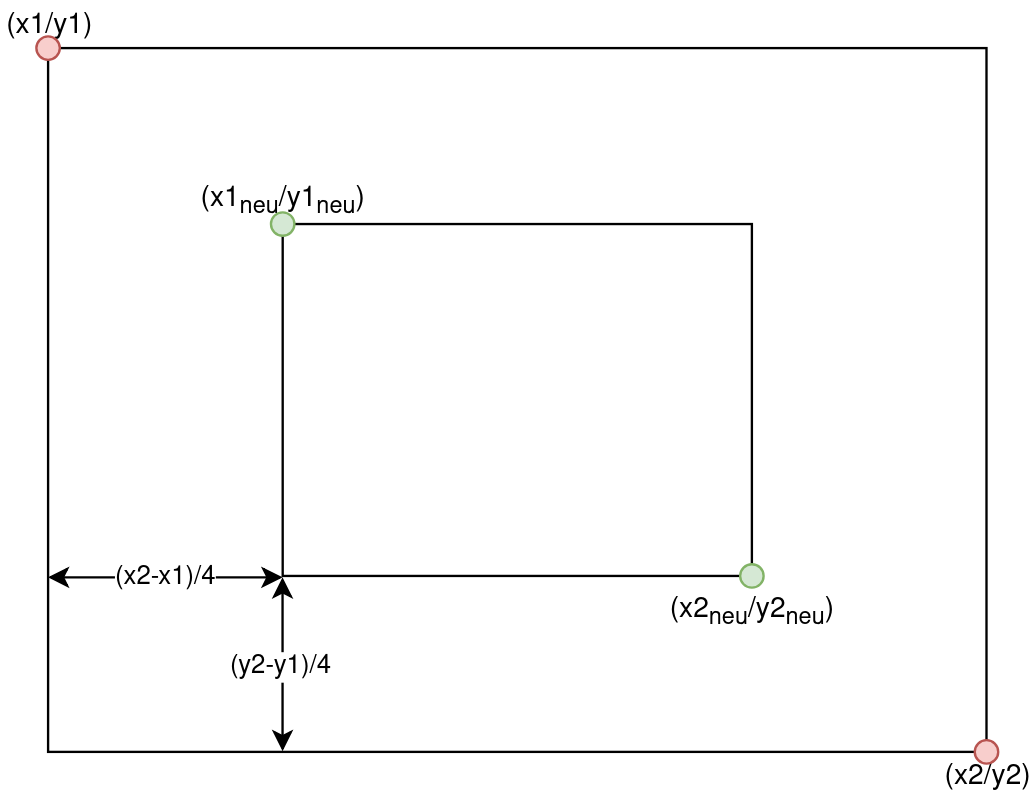
\includegraphics[width=0.7\textwidth]{zoom.png}
	\caption{Debouncer und Input-Modul, schematische Darstellung}
	\label{fig:zoom}
\end{figure}

\section{Clock- und Resetsignal}

\chapter{Ausblick \& Fazit}

% Literaturverzeichnis
\bibliography{bib}{}
\bibliographystyle{unsrt}

\end{document}